%Dokumentklasse

%draft als optionohne bilder für bessere performance
%\documentclass[a4paper,12pt,]{scrreprt}

%normal mit Bildern
\documentclass[
a4paper,
12pt,
draft=True]
{scrartcl}

%Section als Chapter
\RedeclareSectionCommand[%
%beforeskip = -1sp plus -1sp minus -1sp,% kleinster negativer Wert, um den Absatzeinzug nach der Überschrift zu verhindern.
afterskip = 1.5 \baselineskip plus -1sp minus 1sp,
font = \Huge,
]{section}

\usepackage[left= 3cm,right = 3cm, bottom = 3cm,top = 3cm]{geometry}
%\usepackage[onehalfspacing]{setspace}

% ============= Packages =============
% Dokumentinformationen
\usepackage[
pdftitle={Praktikum - Umwelttechnik},
pdfsubject={},
pdfauthor={Roman-Luca Zank},
pdfkeywords={},	
%Links nicht einrahmen
hidelinks
]{hyperref}

%nur Text zum prüfen des Umfangs

% Standard Packages
%\usepackage[bottom]{footmisc}
\usepackage[utf8]{inputenc}
\usepackage[ngerman]{babel}

\usepackage[T1]{fontenc}
%\usepackage{helvet}

%\renewcommand{\familydefault}{\sfdefault}

\usepackage{graphicx}
\graphicspath{{img/}}
\usepackage{mhchem}
\usepackage{fancyhdr}
\usepackage{lmodern}
\usepackage{color}
\usepackage[bottom]{footmisc}
\usepackage{setspace}\usepackage{threeparttable}
%==================================================================
%\begin{threeparttable} 
%	\begin{tabular}{|l|c|r|} 
%		\hline 
%		A & B & C \\
%		\hline
%		1 & 2 & 3 \tnote{1} \\
%		\hline
%	\end{tabular} 
%	\begin{tablenotes}\footnotesize 
%		\item[1] Prognose 2003 
%	\end{tablenotes}
%====================================================================
\usepackage{placeins}
\usepackage{booktabs}
\usepackage{caption}
\usepackage[list=true]{subcaption}
\usepackage{longtable}
\usepackage{tikz}
\usepackage{pgfplots}
\usepackage{lastpage}
%\usepackage{ulem}
\usepackage{mathtools}
\usepackage{adjustbox}
\usetikzlibrary{patterns}
\usepackage{pdfpages}

%Einheitenpackage
\usepackage{siunitx}  
\sisetup{	locale = DE, 
	per-mode=fraction,
	inter-unit-product=\ensuremath{\cdot},
	detect-weight = true,
	quotient-mode=fraction
}
%neue Einheiten definieren
\DeclareSIUnit\xyz{xyz}	
\DeclareSIUnit\rpm{rpm}	
\DeclareSIUnit\mws{mWS}	
\DeclareSIUnit\degrees{^\circ}	

%Automatisch cdot statt *
\DeclareMathSymbol{*}{\mathbin}{symbols}{"01}


%Tabelle
\usepackage{tabularx}
\usepackage{tabulary}

%nur letzte Zeile der Gleichung nummerieren
\makeatletter
\def\Let@{\def\\{\notag\math@cr}}
\makeatother

% zusätzliche Schriftzeichen der American Mathematical Society
\usepackage{amsfonts}
\usepackage{amsmath}

%Abkürzungsverzeichnis
\usepackage{acronym}

%kein Abstand bei neuem Kapitel vom Seitenanfang
%\vspace*{2.3\baselineskip} = ORIGINAL
%\renewcommand*{\chapterheadstartvskip}{\vspace*{.0\baselineskip}}

%nicht einrücken nach Absatz
\setlength{\parindent}{0pt}

\urlstyle{same}


% ============= Kopf- und Fußzeile =============
\pagestyle{fancy}
%
\lhead{}
\chead{}
\rhead{}%\slshape }%\leftmark}
%%
\lfoot{}
\cfoot{}
\rfoot[{\thepage\ of \pageref*{LastPage}}]{Seite \thepage\ von \pageref*{LastPage}}
%%
\renewcommand{\headrulewidth}{0pt}
\renewcommand{\footrulewidth}{0pt}
%\renewcommand{\chapterpagestyle}{fancy}

%Fußnotelinie
%\let\footnoterule

%Fußnote mit Klammer
\renewcommand*{\thefootnote}{(\arabic{footnote})}

%Abb. statt Abbildung
\addto\captionsngerman{%
	\renewcommand{\figurename}{Abb.}%
	\renewcommand{\tablename}{Tab.}%
}

% ============= Package Einstellungen & Sonstiges ============= 
%Besondere Trennungen
%\hyphenation{De-zi-mal-tren-nung}
\usepackage[none]{hyphenat}
\hyphenpenalty=5000
\tolerance=5000
\providecommand\phantomsection{}

\usepackage{mathtools}


% ============= Dokumentbeginn =============

\begin{document}
%Seiten ohne Kopf- und Fußzeile sowie Seitenzahl
\pagestyle{empty}

%\begin{center}
\begin{tabular}{p{\textwidth}}


\begin{center}

\includegraphics[scale=0.75]{logos.jpg}\\
\end{center}


\\

\begin{center}
\LARGE{\textsc{
Protokoll \\
Analytik\\
}}
\end{center}

\\

%\begin{center}
%\large{Fakultät für Muster und Beispiele \\
%der Hochschule Musterhausen \\}
%\end{center}
%
%\\
\begin{center}
	\textbf{\LARGE{Versuch 1.2}}
\end{center}
\begin{center}
\Large{Bestimmung des Wassergehalt von Flüssigkeiten und Feststoffen (Iodometrie)}
\end{center}

\begin{center}
	\large{Gruppe 2.4 (BCUC4)}
\end{center}


\\
%\begin{center}
%zur Erlangung des akademischen Grades\\
%Bachelor of Engineering
%\end{center}


%\begin{center}
%vorgelegt von
%\end{center}

\begin{center}
\Large{\textbf{Teilnehmer:}} \\ 
\end{center}
\begin{center}
\large{Willy Messerschmidt \\
	Roman-Luca Zank} \\
\end{center}


\\

\begin{center}
\begin{tabular}{lll}
%\large{\textbf{Protokollführer:}} & & \large{NAME}\\
&&\\
\large{\textbf{Datum der Versuchsdurchführung:}}&& \large{29.05.2020 (Online)}\\
&&\\
\large{\textbf{Abgabedatum:}}&& \large{???}
\end{tabular}
\end{center}

\\ \\ \\ \\
\large{Merseburg den \today}

\end{tabular}
\end{center}


%\include{14_danksagungen}

%\include{15_zusammenfassung}

% Beendet eine Seite und erzwingt auf den nachfolgenden Seiten die Ausgabe aller Gleitobjekte (z.B. Abbildungen), die bislang definiert, aber noch nicht ausgegeben wurden. Dieser Befehl fügt, falls nötig, eine leere Seite ein, sodaß die nächste Seite nach den Gleitobjekten eine ungerade Seitennummer hat. 
\cleardoubleoddpage

% Pagestyle für Titelblatt leer
\pagestyle{empty}

%Seite zählen ab
\setcounter{page}{0}

%Titelblatt
\begin{center}
\begin{tabular}{p{\textwidth}}


\begin{center}

\includegraphics[scale=0.75]{logos.jpg}\\
\end{center}


\\

\begin{center}
\LARGE{\textsc{
Protokoll \\
Analytik\\
}}
\end{center}

\\

%\begin{center}
%\large{Fakultät für Muster und Beispiele \\
%der Hochschule Musterhausen \\}
%\end{center}
%
%\\
\begin{center}
	\textbf{\LARGE{Versuch 1.2}}
\end{center}
\begin{center}
\Large{Bestimmung des Wassergehalt von Flüssigkeiten und Feststoffen (Iodometrie)}
\end{center}

\begin{center}
	\large{Gruppe 2.4 (BCUC4)}
\end{center}


\\
%\begin{center}
%zur Erlangung des akademischen Grades\\
%Bachelor of Engineering
%\end{center}


%\begin{center}
%vorgelegt von
%\end{center}

\begin{center}
\Large{\textbf{Teilnehmer:}} \\ 
\end{center}
\begin{center}
\large{Willy Messerschmidt \\
	Roman-Luca Zank} \\
\end{center}


\\

\begin{center}
\begin{tabular}{lll}
%\large{\textbf{Protokollführer:}} & & \large{NAME}\\
&&\\
\large{\textbf{Datum der Versuchsdurchführung:}}&& \large{29.05.2020 (Online)}\\
&&\\
\large{\textbf{Abgabedatum:}}&& \large{???}
\end{tabular}
\end{center}

\\ \\ \\ \\
\large{Merseburg den \today}

\end{tabular}
\end{center}
 %Prokolle
%\begin{center}
\begin{tabular}{p{\textwidth}}


\begin{center}

\includegraphics[scale=0.75]{img/logos.jpg}\\
\end{center}


\\

\begin{center}
\LARGE{\textsc{
Recherche \\
Rückgewinnung von Ammoniak aus Industrieabwässern\\
}}
\end{center}

%\begin{center}
%\large{Fakultät für Muster und Beispiele \\
%der Hochschule Musterhausen \\}
%\end{center}
%
%\\
 \\
 
\begin{center}
\textbf{\Large{Seminararbeit in Medienrecherche}}
\end{center}

\begin{center}
	\large{im WiSe 2019}
\end{center}
 \\
%\begin{center}
%zur Erlangung des akademischen Grades\\
%Bachelor of Engineering
%\end{center}


\begin{center}
\large{vorgelegt von}
\end{center}
\\


\begin{center}
\Large{\textbf{Roman-Luca Zank}} \\
\end{center}

\begin{center}
3. Semester \\
Chemie- und Umwelttechnik \\
\end{center}


\begin{center}
\begin{tabular}{lll}
	\textbf{E-Mail:} & & romanzank@mail.de\\
	\textbf{Matrikelnummer:} & &25240\\
	\textbf{Adresse:} & &Platz der Bausoldaten 2, Zimmer 224\\
	\textbf{Ort:} & &06217 Merseburg\\
	&& \\
	\textbf{Prüfer:} & & Dr. Frank  Baumann\\
\end{tabular}
\end{center}

\\ \\ \\ \\ \\
\large{Merseburg, \today}

\end{tabular}
\end{center}
 %Seminar-/Abschlussarbeit

% Pagestyle für Rest des Dokuments
\pagestyle{fancy}

%Inhaltsverzeichnis
\tableofcontents
\thispagestyle{empty}

%Inhalt
%
%Verzeichnis aller Bilder
\label{sec:bilder}
\listoffigures
\addcontentsline{toc}{chapter}{Abbildungsverzeichnis}
\thispagestyle{empty}

%Verzeichnis aller Tabellen
\label{sec:tabellen}
\listoftables
\addcontentsline{toc}{chapter}{Tabellenverzeichnis}
\thispagestyle{empty}



%%Abkürzungsverzeichnis
%\setlength{\columnsep}{20pt}
%\twocolumn
%\addchap{Nomenklatur}
%\label{sec:abkurzung}
%\begin{acronym}
%\acro{kf}[$\text{k}_\text{f}$]{Durchlässigkeitsbeiwert}
%\acro{t}{Durchlaufzeit}
%\acro{tm}[$\text{t}_\text{m}$]{Mittlere Durchlaufzeit}
%\acro{V}{Volumen}
%\acro{h}{Höhe der Wassersäule}
%\acro{Q}{Volumenstrom}
%\acro{l}{Durchströmte Länge}
%\acro{A}{Grundfläche}
%\acro{d}{Durchmesser}
%
%\end{acronym}
%\subsubsection{Aufrufen einer Abkürzung}
%\acs{rT}
%\begin{verbatim}
%\acs{Abkürzung}
%\end{verbatim}

%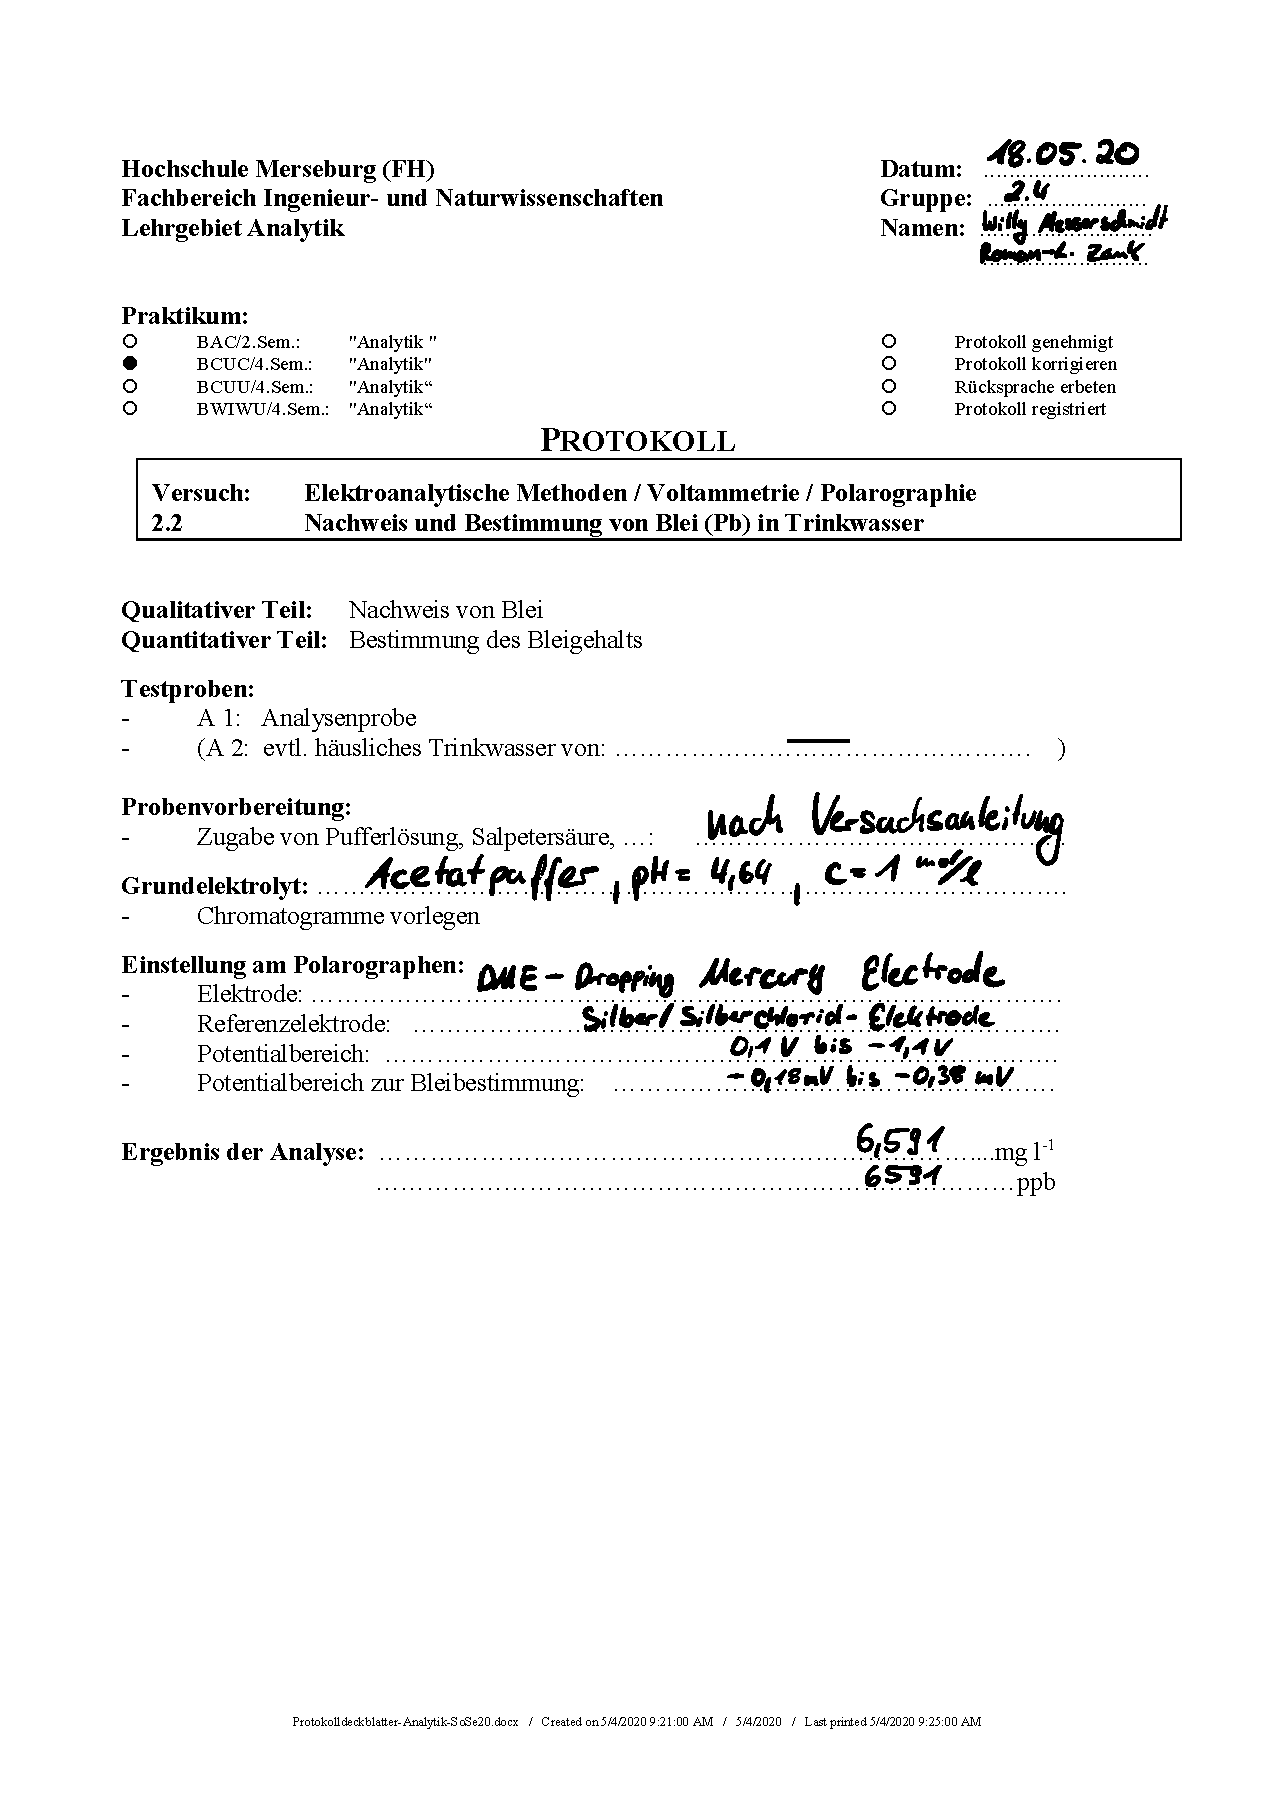
\includepdf[]{Deckblatt}
\pagebreak
\section{Einleitung}
\label{sec:einleitung}
Der Wassergehalt von flüssigen und festen Werk-, Betriebs- und Hilfsstoffen muss für ihre technische Anwendung in vielen Bereichen gemessen werden. Ein Bestimmungsverfahren stellt dabei die \textsc{Karl-Fischer}-Titration dar. Im Verlauf des hier beschriebenen Praktikumsversuches wurde eine Flüssigkeitsprobe und eine Feststoffprobe analysiert.
\subsection{Aufgaben:}
\begin{itemize}
	\item Versuchen Sie den angezeigten bzw. Ausgedruckten Titer (mg Wasser/mg Titrierlösung) nachzurechnen. Können Sie die Berechnung nachvollziehen ?
\end{itemize}







\section{Theorie}
\label{sec:theorie}

\subsection{Voltammetrie}
Voltammetrie ist eine Sammelbezeichnung für einige elektrochemische Analysemethoden, bei denen die Spannung (das Potential) und der fließende Strom zwischen mindestens zwei Elektroden betrachtet werden, um daraus Aussagen zur Zusammensetzung einer Probe abzuleiten.\\
Die \textit{Voltammetrie} ist nicht mit der \textit{Voltametrie} zu verwechseln. Bei letzterer wird lediglich die Spannung gemessen.
\subsection{Die Elektrochemische Spannungsreihe}


Die Elektrochemische Spannungsreihe ordnet Metalle nach ihrem elektrochemischen Potential. Als Bezug dient dabei stets die Standardwasserstoffelektrode. In Verbindung letzterer Halbzelle mit einem Metall, in seiner einmolaren Metallsalzlösung bei Standardbedingungen, kann das Standardpotential des Metalls als anliegende Spannung zwischen den Elektroden gemessen werden. Das Vorzeichen der Standardpotentiale sagt aus, in welche die Richtung Elektronen strömen. Es besteht ein direkter Zusammenhang zwischen dem Standardelektrodenpotential eines Metalls und dessen Bestreben reduziert zu werden. Je größer das Elektrodenpotential ist, umso edler ist auch das Metall und umso eher wird es reduziert. Verwendung findet dieser Umstand zum Beispiel in der Berechnung galvanischer Elemente. Im folgenden kann anhand der Standardelektrodenpotentiale gelöster Metallionen deren Positionierung in einem Polarogramm abgeleitet werden.\cite{spannungsreihe}\\

\vline

\subsection{Analyse der Polarogramme}
Grundlage für die Analyse der enthaltenen Metall-Ionen ist die aufgenommene Strom-Spannungs-Kurve des Polarographen. Aufgrund der spezifischen Halbstufenpotentiale von Metall-Ionen ändert sich bei unterschiedlichen Arbeitspotentialen die gemessene Stromstärke. Dieser Strom an der Arbeitselektrode 
tritt als Folge der Reduktionsreaktion der Metall-Ionen auf und ist direkt proportional zur Konzentration des umgesetzten Stoffes. Der Strom im Zusammenhang mit diesem Massentransport der Ionen wird als \textsc{Faraday}scher Strom bezeichnet. \linebreak Um eine ausreichende Leitfähigkeit und somit einen entsprechenden Ladungstransport in der Lösung garantieren zu können, werden den untersuchten Proben oft Grundelektrolyten in Form von Salzen, Säuren oder Basen zugegeben.\linebreak
Aufgrund der spezifischen Halbstufenpotentiale lassen sich qualitative Ergebnisse dieses Verfahrens auswerten. Betrachtet man jedoch auch den Zusammenhang des Stromflusses bei einem bestimmten Arbeitspotential mit der Konzentration des umgesetzten Stoffes, so lassen sich ebenfalls quantitative Bewertungen äußern.\linebreak
Für diese Betrachtung ist jedoch eine Form der Kalibrierung notwendig, um die gemessenen Signale quantitativ auswerten zu können. Dies ist zum einen über einen externen oder internen Standard möglich, jedoch wurde sich aufgrund der geringen zu bestimmenden Konzentrationen in diesem Versuch für die Aufstockmethode, auch Standardadditionsmethode genannt, entschieden. Möchte man einen internen oder externen Standard nutzen so sind in diesem Fall ebenfalls Kalibrierkurven mit linearem Zusammenhang mittels bekannter Referenz aufzustellen.\linebreak
Bei dieser Methode wird in diesem Versuch nach der polarographischen Analyse der unbehandelten Probe, eine definierte Menge eines bekannten Standards zugegeben. Dieser Standard enthält dabei den zu bestimmenden Stoff in einer exakt bekannten Konzentration. Aus den gemessenen Datenpunkten lässt sich nun eine Geradengleichung bestimmen (siehe Abb. \ref{fig:standardaddition} und Gl. \ref{gl:1}).

\begin{flalign}
\label{gl:1}
Y &= \frac{\Delta y}{\Delta x}*X+yA
\end{flalign}

%%Start
%\begin{figure}[h!]
%	\centering
%	\includegraphics[width=0.5\textwidth]{img/Standardaddition}
%	\caption{Darstellung der Standardadditionsmethode \cite{}}
%	\label{fig:standardaddition}
%\end{figure}
%\FloatBarrier
%%Ende

Aus der ermittelten Geradengleichung, lässt sich nun, aufgrund der geometrischen Beziehung der Strahlensätze, die Konzentration der Probe über den Wert $xA$ in Abb. \ref{fig:standardaddition} bestimmen. Eine Herleitung dazu ist unter Gl. \ref{gl:2} und Gl. \ref{gl:3} zu finden. Die Bedeutungen der Variablen sind nachfolgend in der Tabelle \ref{tab:variablen} aufgeführt.

\begin{flalign}
\label{gl:2}
	Y &= \frac{y}{x}*X+yA\\
	X&= \frac{Y-yA}{\frac{y}{x}}
\end{flalign}

\textit{Für $Y=0$ heißt das:}

\begin{flalign}
\label{gl:3}
X&= xA = \frac{0-yA}{\frac{y}{x}} = \frac{-yA}{\frac{y}{x}}\\
xA&= -c\\
c	&= \underline{\underline{\frac{yA}{\frac{y}{x}}}}
\end{flalign}

\vspace*{-5mm}

%Tabelle START
\renewcommand{\arraystretch}{1.2}
\begin{table}[h!]
	\centering
	%\caption{Variablen der Abb.\ref{fig:standardaddition} und der Tab.\ref{tab:variablen} und ihre Bedeutungen}
	\caption{Variablen und ihre Bedeutung}
	\label{tab:variablen}
	%\makebox[\textwidth]{
	%	\resizebox{17cm}{!}{
			\begin{tabular}{c|c}
				\hline
				\textbf{Variable}&\textbf{Bedeutung} \\
				\hline
				A& Analyt \\
				Z& Zugabe\\
				$Y$& Signalwert\\
				$yA$& Signalwert der Testlösung - nur Analyt\\
				$\Delta y$& Signaländerungnach Zugabe der Standardlösung \\
				$X$& Analytwert\\
				$xA$&Analytkonzentration in der Testlösung\\
				$\Delta x$& Konzentrationsändeung durch Standard-Zugabe \\
				\hline	
			\end{tabular}
		%	}
			%}
		\end{table}
		\FloatBarrier
		\vspace*{-2.5mm}
		%Tabelle Ende


\newpage
\section{Geräte und Chemikalien}
\label{sec:geraete}

\textbf{Geräte:}
\begin{itemize}
\item Trockenofen Mettler-Toledo DO-302
\item Waage
\item Titrator T50, \textsc{Karl-Fischer}-Titrator (Fa. Mettler)
\item Computer mit Software \textsc{LabX}
\item Mikroliterspritze
\end{itemize}

\vspace*{5mm}

\textbf{Proben/Chemikalien:}
\begin{itemize}
\item \textsc{Karl-Fischer}-Reagenz (Einkomponentig)
\item deionisiertes Wasser
\item Isopropanol (2-Propanol)
\item Polyamid

\end{itemize}







\section{Durchführung}
\label{sec:durchfuerung}
Tatsächlich wurde das Praktikum nicht durch die Autoren dieses Protokolls durchgeführt. Aus diesem Grund wird an dieser Stelle auf die Beschreibung der Versuchsdurchführung in der Angehängten Praktikumsanweisung verwiesen.

\newpage


\section{Ergebnisse und Berechnungen}
\label{sec:ergebnisse}
%Tabelle START

	\vspace*{-2.5mm}
	\renewcommand{\arraystretch}{1.2}
	\begin{table}[h!]
		\centering
		\caption{Messwerte zur Titerbestimmung}
		\label{tab:MesswerteTiterbestimmung}
			%\resizebox{17cm}{!}{
		\begin{tabulary}{\textwidth}{|C|C|C|C|C|C|C|}
		\hline
		\multicolumn{7}{|c|}{Automatisch }\\
			\hline
			\textbf{Probengröße Wasser} [\si{\gram}]& \textbf{Konz.} [\si{\milli\gram\per\milli\liter}]& \textbf{Titer} &\textbf{DRIFT} [\si{\micro\gram\per\minute}]&\textbf{DRIFT} [\si{\micro\liter\per\minute}]&\textbf{Dauer} [min]&\textbf{V$_{EQ}$} [\si{\milli\liter}]\\
			\hline
			0,005& 4,81040 &0,962&4,3&0,7&1,55&1,0405
			\\
			\hline
			0,005& 5,18954 &1,038&1,1&0,2&1,37&0,96375
			\\
			\hline
			0,005& 5,68201&1,136&&&&\\
			\hline
			\hline
			\textbf{Mittelwert}&5,227&1,045 &&&&\\
			\cline{1-3}
			\textbf{Standard\-abweichung}&0,437&0,0874
			&&&&\\
			\cline{1-3}
			\textbf{rel.Strd.\-abweichung}&8,361\%&8,361\% &&&&\\
			\hline
		
		\end{tabulary}
	%	}
	\end{table}
	\FloatBarrier 
	% \vspace*{-2.5mm}
	%Tabelle ENDE
   
%Tabelle START
 
  \vspace*{-2.5mm}
 \renewcommand{\arraystretch}{1.2}
 \begin{table}[h!]
 	\centering
 	\caption{Messwerte zur Isopropanol-Probe}
 	\label{tab:MesswerteIsopropanol}
 %	\resizebox{17cm}{!}{
 	\begin{tabulary}{\textwidth}{|C|C||C|C|C|}
 		\hline
 		\multicolumn{5}{|c|}{Automatisch }\\
 		\hline
 		\textbf{Probengröße Isopropanol} [\si{\gram}]& \textbf{m\% \ce{H2O}}& \textbf{m(\ce{H2O})} [\si{\milli\gram}]&\textbf{DRIFT} [\si{\micro\gram\per\minute}]&\textbf{DRIFT} [\si{\micro\liter\per\minute}]\\
 		\hline
 		0,4037& 0,0036 &0,0145&28,6&5,5\\
 		\cline{1-3}
 		0,3716& 0,3553 &1,2303&&\\
 		\hline
 		\hline
 	\textbf{Mittelwert}&0,1795&0,6674 &&\\
 	\cline{1-3}
 	\textbf{Standard\-abweichung}&0,2487&0,9233&&\\
 	\cline{1-3}
 	\textbf{rel.Strd.\-abweichung}&138,552\%&138,342\% &&\\
 	\hline
 	\hline
 \textbf{Versuchszeit}&\multicolumn{4}{|c|}{1,18\si{\minute}} \\
 \hline
 \end{tabulary}
 	%}
 \end{table}
 \FloatBarrier 
% \vspace*{-2.5mm}
 %Tabelle ENDE


%Tabelle START
\vspace*{-2.5mm}
\renewcommand{\arraystretch}{1.2}
\begin{table}[h!]
	\centering
	\caption{Messwerte zur Isopropanol-Probe/2-Propanol}
	\label{tab:Messwerte2Propanol}
	%	\resizebox{17cm}{!}{
	\begin{tabulary}{\textwidth}{|C|C||C|}
		\hline
		\multicolumn{3}{|c|}{Automatisch }\\
		\hline
		\textbf{Probengröße Isopropanol} [\si{\gram}]& \textbf{m\% \ce{H2O}}& \textbf{m(\ce{H2O})} [\si{\milli\gram}]\\
		\hline
		0,7401& 0,0435&0,3219\\
		\cline{1-3}
		0,08851& 0,0384 &0,3399\\
		
		\cline{1-3}
		0,9157& 0,0431 &0,3947\\
		\cline{1-3}
		0,9442& 0,0379 &0,3579\\
		
		\hline
		\hline
		\textbf{Mittelwert}&0,0407&0,3536 \\
		\cline{1-3}
		\textbf{Standard\-abweichung}&0,0030&0,0311\\
		\cline{1-3}
		\textbf{rel.Strd.\-abweichung}&7,3292\%&8,7855\% \\
		\hline
		
	\end{tabulary}
	%}
\end{table}
\FloatBarrier 
% \vspace*{-2.5mm}
%Tabelle ENDE

%Tabelle START
\vspace*{-2.5mm}
\renewcommand{\arraystretch}{1.2}
\begin{table}[h!]
	\centering
	\caption{Messwerte zur Polyamid-Probe}
	\label{tab:MesswertePoliamid}
	%	\resizebox{17cm}{!}{
	\begin{tabulary}{\textwidth}{|C|C||C|}
		\hline
		\multicolumn{3}{|c|}{Automatisch }\\
		\hline
		\textbf{Probengröße Polyamid} [\si{\gram}]& \textbf{m\% \ce{H2O}}& \textbf{m(\ce{H2O})} [\si{\milli\gram}]\\
		\hline
		0,1996& 2,3217&4,6341\\
		\cline{1-3}
		0,2028& 1,9189 &3,8915\\
		
		\hline
		\hline
		\textbf{Mittelwert}&2,1203&4,2628 \\
		\cline{1-3}
		\textbf{Standard\-abweichung}&0,2848&0,5251\\
		\cline{1-3}
		\textbf{rel.Strd.\-abweichung}&13,4331\%&12,3178\% \\
		\hline
		
	\end{tabulary}
	%}
\end{table}
\FloatBarrier 
% \vspace*{-2.5mm}
%Tabelle ENDE
\subsection{Manuelle Berechnung der relativen Standardabweichung}
Die Berechnung der relativen Standardabweichung von Hand, erfolgt analog der Gleichung (\ref{gl:S_rel}). Die mit dem Taschenrechner erhaltenen Ergebnisse sind in den Tabellen \ref{tab:MesswerteTiterbestimmung} bis \ref{tab:MesswertePoliamid} in der Sektion \glqq Manuell\grqq  \, aufgeführt. 
\begin{flalign}\label{gl:S_rel}
	s_{rel}&=\frac{s}{\bar{x}}\\
	&=\frac{0,2848\%}{2,1203\%}\\
	&=0,134321=\underline{\underline{13,4321\%}}
\end{flalign}

\subsection{Manuelle Titerbestimmung}
Die Berechnung des Titers $t$ der KF-Lösung ist in Gleichung (\ref{gl:titer}) beispielhaft für ein Wertepaar dargestellt. Die verwendeten Werte entstammen der ersten Zeile der Tabelle \ref{tab:MesswerteTiterbestimmung}.
\begin{flalign}\label{gl:titer}
	t&=\frac{c_{ist}}{c_{soll}}\\
	&=\frac{\SI{4,81040}{\milli\gram\per\milli\liter}}{\SI{5,0}{\milli\gram\per\milli\liter}}\\
	&=\underline{\underline{0,96208}}
\end{flalign}
\subsection{Manuelle Bestimmung des Wassergehaltes}

\newpage
\section{Diskussion}
\label{sec:diskussion}


\subsection{Bedeutung der Driftkorrektur}
Der Drift wurde als linearer Zusammenhang vom Messgerät durch Kalibrierung erfasst. Die Einbeziehung des Massen- und Volumendrifts erlaubt es die wiederkehrende Abweichung des Messgerätes zu berücksichtigen und damit eine größere Genauigkeit des erhaltenen Ergebnisses. Eine absolute Abweichung wird dabei durch Multiplikation mit der Messdauer erhalten.



\subsection{Bewertung der Feuchtigkeit}

\textbf{Isopropanol/2-Propanol}\\
Die Feuchtigkeitsmesswerte des Isopropanols sind in der Tabelle \ref{tab:Messwerte2Propanol} einzusehen. Der mittlere gemessene Wassergehalt von 0,0407\% ist sehr gering. Isopropanol ist in jedem Verhältnis mit Wasser mischbar und somit ist das Lösen von Luftfeuchtigkeit nicht auszuschließen.\cite{isopropanol} Zudem ist Isopropanol auch im Handel mit $99,95\%$ Reinheit erhältlich, was die gemessenen $0,04\%$ Wassergehalt bestätigen könnte.\cite{isoprop} Daher ist der Messwert plausibel.\\

\textbf{Polyamid}\\
Die Feuchtigkeitsmesswerte des Polyamids sind in der Tabelle \ref{tab:MesswertePoliamid} einzusehen. Der mittlere gemessene Wassergehalt von 2,1203\% ist deutlich höher als beim Isopropanol. Dieser Unterschied basiert auf der Zusammensetzung des Polyamid und ist abhängig von dessen Konzentration an Amidgruppen im kristallinen Gefüge. Somit kommt des dazu, dass bei Umgebungsluft Polyamid je nach genauem Gefüge und je nach betrachteter Quelle, beispielsweise bei PA 6, $2,5-3,5\%$ Wassergehalt möglich sind.\cite{Wikipedia.2020,Kaiser.2006} Als Gegenbeispiel besitzt PA 12 bei Umgebungsluft einen Wassergehalt von $0,2-0,5\%$.\cite{Wikipedia.2020} Je nachdem welche Art von Polyamid-Probe untersucht wurde erscheint der Messwert als mehr oder weniger plausibel.\\

\textbf{Risiken von Wasser bei der Polymerverarbeitung}\\
Die gebräuchlichsten Alltagspolymere sind Thermoplaste. Sie werden zur Verarbeitung und Umformung meist erwärmt. Wie die Polyamid-Probe zeigt können Kunststoffe schon bei Umgebungsluft in geringen Mengen aufnehmen. Das hat zur Folge, dass ähnlich wie beim Werkstoff Holz, der Kunststoff aufquellen kann. Eine mögliche Folge ist, dass sich Bauteile einer Volumenzunahme von 0,3 \% pro 1 \% Wasseraufnahme zur Folge haben können.\cite{Kaiser.2006} Je nach Einsatzgebiet könne  hierbei Stabilität und Sicherheit gefährdet sein. Im selben Zusammenhang können sich durch das Quellen oder Schwinden des Kunststoffes Einschlüsse bilden, welche ebenfalls den Kunststoff in seiner Struktur verändern können. Betrachtet man Wasser nicht nur als Quell- sondern auch als Lösungsmittel so ist durchaus auch eine Extraktion von Inhaltsstoffen, wie Additive möglich, welche den Kunststoff nachhaltig verändern können. Auch die Veränderung von weiteren physikalischen Eigenschaften ist dabei möglich, wie zum Beispiel die Veränderung der Leitfähigkeit.\cite{polymermerse} 

\section{Fehlerbetrachtung}
\label{sec:fehler}

Die zur Auswertung zugeteilten Werte waren zum Teil kaum auswertbar. Daher sind in den Tabellen des Kapitels \ref{sec:ergebnisse} sind einige Lücken zu erkennen. Die Auswertung der Messungen einiger Ethanol-Proben wurde unmöglich. Teilweise sind Messergebnisse auch nicht nachvollziehbar. So zum Beispiel die enorme Differenz zwischen den Messungen der Isopropanol-Probe in Tabelle \ref{tab:MesswerteIsopropanol}. Unklar ist warum man für den gleichen Stoff, 2-Propanol, auch Isopropanol genannt, zwei unterschiedliche Namen verwendet und sie in separaten Versuchen untersucht hat. 

Dadurch, dass der Versuch nicht von den Autoren selbst durchgeführt wurde sind Rückschlüsse auf eventuell geschehene Missgeschicke oder grobe Anwendungsfehler, die die gefundenen Diskrepanzen erklären könnten, kaum mehr möglich. 

Messungenauigkeiten der Waage und der Mikroliterspritze können, wie auch Messfehler des Titrators, einen gewissen Fehler verursacht haben. Viel entscheidender erscheinen allerdings die Anwendungsfehler. Diese erstrecken sich von Übertragungsfehlern zu Abweichungen in der Handlungsreihenfolge oder der nicht-Einhaltung von vorgegebenen Zeiten und Hinweisen.

Ebenfalls ist nicht klar ob bei der Analyse mit der Ofentechnik alle Bauteile, die die Probe enthalten, luftdicht verschlossen waren. War dies nicht gegeben, könnte der Wassergehalt durch Wasserverlust an die Umgebung oder zusätzliche Luftfeuchte verfälscht werden.

Auch verunreinigte oder überalterte Geräte und Chemikalien könnten Abweichungen verursacht haben.

Insgesamt ist es ratsam den Versuch erneut durchzuführen, um die möglichen Anwendungsfehler dieser Versuchsdurchführung ausschließen zu können.

%\section*{Anhang}
\addcontentsline{toc}{section}{Anhang}
%\label{sec:anhang}
 
 
 
 

%Praktikumsskript, Modul ………, Versuch …….., Prof. Musterprof. 
%DIN 12345, Jahr der Veröffentlichung 
%Link der Internetseite, Zugriffsdatum 
%Buchtitel, Autor, Verlag, Veröffentlichungsjahr 

%Literaturverzeichnis Bücher
\bibliography{Literatur}
\bibliographystyle{unsrtdin}
\addcontentsline{toc}{section}{Literaturverzeichnis}

https://www.analytics-shop.com/de/sa278475-2l-de.html

Isopopranol nachweis wasser


https://de.wikipedia.org/wiki/Polyamide
http://www.kunststoffe.de/themen/basics/technische-kunststoffe/polyamide-pa/artikel/polyamide-pa-651963
https://wiki.polymerservice-merseburg.de/index.php/Wasseraufnahme

Nachweis für PA

%\chapter*{Eidesstattliche Erklärung}
\label{erklaerung}
Hiermit versichere ich, die vorliegende Seminararbeit selbstständig und nur unter Verwendung der von mir angegebenen Quellen und Hilfsmittel verfasst zu haben. Sowohl inhaltlich als auch wörtlich entnommene Inhalte wurden als solche kenntlich gemacht. Die Arbeit hat in dieser oder vergleichbarer Form noch keinem anderem Prüfungsgremium vorgelegen. \\
\\[1.5cm]
Datum:	\hrulefill\enspace Unterschrift: \hrulefill
\\[3.5cm]
\addcontentsline{toc}{chapter}{Selbstständigkeitserklärung}

\end{document}
